\index{PSHA!Input model}
An OpenQuake PSHA input model contains four distinct information blocks: (1) information regarding location, geometry, and seismicity properties of seismic sources, (2) information about ground motion prediction equations to be  adopted in the calculation, (3) information about the epistemic uncertainties related to the two aforementioned points, and (4) information specifying calculation settings.

The description of epistemic uncertainties is accomplished via a logic-tree 
structure, described branching level by branching level. In particular, OpenQuake requires two logic-tree structures, one describing epistemic uncertainties associated with the creation of the ERF - called Seismic Source logic tree - and one considering the uncertainties connected with the use of GMPEs - called GMPE logic tree. 
%
\index{Logic Tree!Seismic source}
\index{Logic Tree!GMPE}
%
Indeed, the OpenQuake PSHA input models are always defined using two logic tree structures. In cases when epistemic uncertainties are non accounted for, the logic tree structure simply have one branching level with just one branch (with weight equal to 1).
%
With respect to the Seismic Source logic tree, we call Source System the object containining the information necessary for the creation of a Source Model considering the epistemic uncertainties on seismic source geometries and parameters. This information consists on a logic tree structure and one - or many - Initial Source Model.
%
Further explanations about the way we describe and model logic-trees are provided in section \ref{hazard:logic_tree} at page \pageref{hazard:logic_tree}. 

The description of OpenQuake seismic source properties is subdivided into 
source location and geometry and source frequency-magnitude distribution.
%
Section \ref{hazard:seismic_source_types} provides an in deep description of 
the properties pertinent to the different source types supported. 

The selection of ground motion prediction equations (GMPE) in OpenQuake 
is basically accomplished by specifying a label in a particular file.  
The user can associate a GMPE to each tectonic region considered in the 
analysis (Active Shallow tectonic, Stable Continental etc.). Examples of 
GMPEs selection are provided in section \ref{hazard:gmpe_selection} at page 
\pageref{hazard:gmpe_selection}.

The last, but not less important, block of information characterizing a PSHA 
input model contains parameters specifying the way calculations must be 
carried out. The information to be included in this part of the input is 
strictly related to the calculation properties of the engine. Section 
\ref{hazard:calculation_settings} provides an outlook of the hazard specific 
calculation setting supported by OpenQuake. 
%
% ------------------------------------------------------------------------------
\section{Logic-tree description}
\label{hazard:logic_tree}
Logic-trees are a tool designed to consider in a systematic manner the 
epistemic uncertainties of models and parameters included in a hazard 
analysis.

In OpenQuake, the description of a logic-tree structure uses as its principal 
component a branching level where a branching level consists on (1) the 
definition of the parameter - or model - affected by uncertainty, (2) the 
specification of the type of uncertainty (3) the listing of the - mutually 
exclusive and collectively exhaustive \citep{bommer2008} - alternative 
hypotheses and, (4) the index of the branches of the previous level to which 
this branching level applies.
%
Each hypothesis (i.e. branch) included in a branching level has an associated value and a corresponding weight expressing - according to different interpretations available in the literature - ``probabilities or simply subjective indications of relative merit'' \citep[][pagecon 999]{bommer2008}.

Figure \ref{fig:logic_tree_branching_levels} depicts a 
branching level defining epistemic uncertainties on the dip angle of simple 
fault sources. In this case the possible values of the dip are specified
on each branch composing the branching level (i.e. 30, 45 and 60 degrees). This 
means that these three values are the only ones admitted for all the sources 
included in the Source Model considered in this example. 
% . . . . . . . . . . . . . . . . . . . . . . . . . . . . . . . . . . . > Figure
\renewcommand{\psedge}{\ncdiag[armA=0,angleB=180,armB=1cm]}
\begin{figure}[!hb]
%\fbox{\begin{minipage}{\textwidth}
\hfill \\
\textcolor{blue01}{\emph{Branching level definition}}: \dotfill Simple Fault 
	Dip Angle \\
\textcolor{blue01}{\emph{Branching level uncertainty type}}: \dotfill 
	Absolute values \\
\textcolor{blue01}{\emph{Applies to}}: \dotfill Simple faults \\
\textcolor{blue01}{\emph{Correlated branches}}: \dotfill Yes \\
\hfill \\
	\centering
	\begin{psTree}[treemode=R,levelsep=*2cm]
			{\Tr{ }}
		\begin{psTree}[treemode=R]{
			\Tr{\parbox[b]{4cm}{ value = 30$^\circ$ 
				\newline weight=w$_1$}}}%
		\end{psTree}%
		\begin{psTree}[treemode=R,treenodesize=1cm]{
			\Tr{\parbox[b]{4cm}{ value = 45$^\circ$ 
				\newline weight=w$_2$}}}%
		\end{psTree}%
		\begin{psTree}[treemode=R]{
			\Tr{\parbox[b]{4cm}{ value = 60$^\circ$ 
				\newline weight=w$_3$}}}%
		\end{psTree}%
	\end{psTree}%
\\ \hfill \\
%\end{minipage}} % End of fbox
\caption{Branching level description example. The upper example shows a 
branching level describing epistemic uncertainties on faults dip angle}
\label{fig:logic_tree_branching_levels}
\end{figure}
% . . . . . . . . . . . . . . . . . . . . . . . . . . . . . . . . . . . < Figure
%

As in the case of Figure \ref{fig:logic_tree_branching_levels},  
Figure \ref{fig:logic_tree_branching_levels_1} also shows a branching level 
defining epistemic uncertainties on the dip angle of simple fault sources.
However - contrary to the example in Figure 
\ref{fig:logic_tree_branching_levels}, in this case the values specified for 
each branch aren't absolute dip angles but instead delta values to be added - 
or subtracted - to the initial dip value specified for each simple fault source
inclued in the initial source model.

% . . . . . . . . . . . . . . . . . . . . . . . . . . . . . . . . . . . > Figure
\renewcommand{\psedge}{\ncdiag[armA=0,angleB=180,armB=1cm]}
\begin{figure}
%\fbox{\begin{minipage}{\textwidth}
\hfill \\
\textcolor{blue01}{\emph{Branching level definition}}: \dotfill
	Simple Fault Dip Angle \\
\textcolor{blue01}{\emph{Branching level uncertainty type}}: \dotfill
	Relative values \\
\textcolor{blue01}{\emph{Applies to}}: \dotfill
	All previous branches \\
\textcolor{blue01}{\emph{Correlated branches}}: \dotfill Yes \\
\hfill \\
	\centering
	\begin{psTree}[treemode=R,levelsep=*2cm]
			{\Tr{ }}
		\begin{psTree}[treemode=R]{
			\Tr{\parbox[b]{4cm}{ value = -15$^\circ$ 
				\newline weight=w$_1$}}}%
		\end{psTree}%
		\begin{psTree}[treemode=R,treenodesize=1cm]{
			\Tr{\parbox[b]{4cm}{ value = 0$^\circ$ 
				\newline weight=w$_2$}}}%
		\end{psTree}%
		\begin{psTree}[treemode=R]{
			\Tr{\parbox[b]{4cm}{ value = +15$^\circ$ 
				\newline weight=w$_3$}}}%
		\end{psTree}%
	\end{psTree}%
\\ \hfill \\
%\end{minipage}} % End of fbox
\caption{Branching level description example. The upper example shows a 
branching level describing epistemic uncertainties on faults dip angle}
\label{fig:logic_tree_branching_levels_1}
\end{figure}
% . . . . . . . . . . . . . . . . . . . . . . . . . . . . . . . . . . . < Figure
%
Once a set of branching levels are defined, they can be easily and flexibly 
combined to create an entire logic-tree structure.
	\marginpar{marco: we probably need abstract classes for all these 
	components of the LT structure}
Figure \ref{fig:logic_tree_schema} shows an example of a logic tree structure 
obtained by combining two distinct branching levels.  

%
% . . . . . . . . . . . . . . . . . . . . . . . . . . . . . . . . . . . > Figure
\begin{figure}
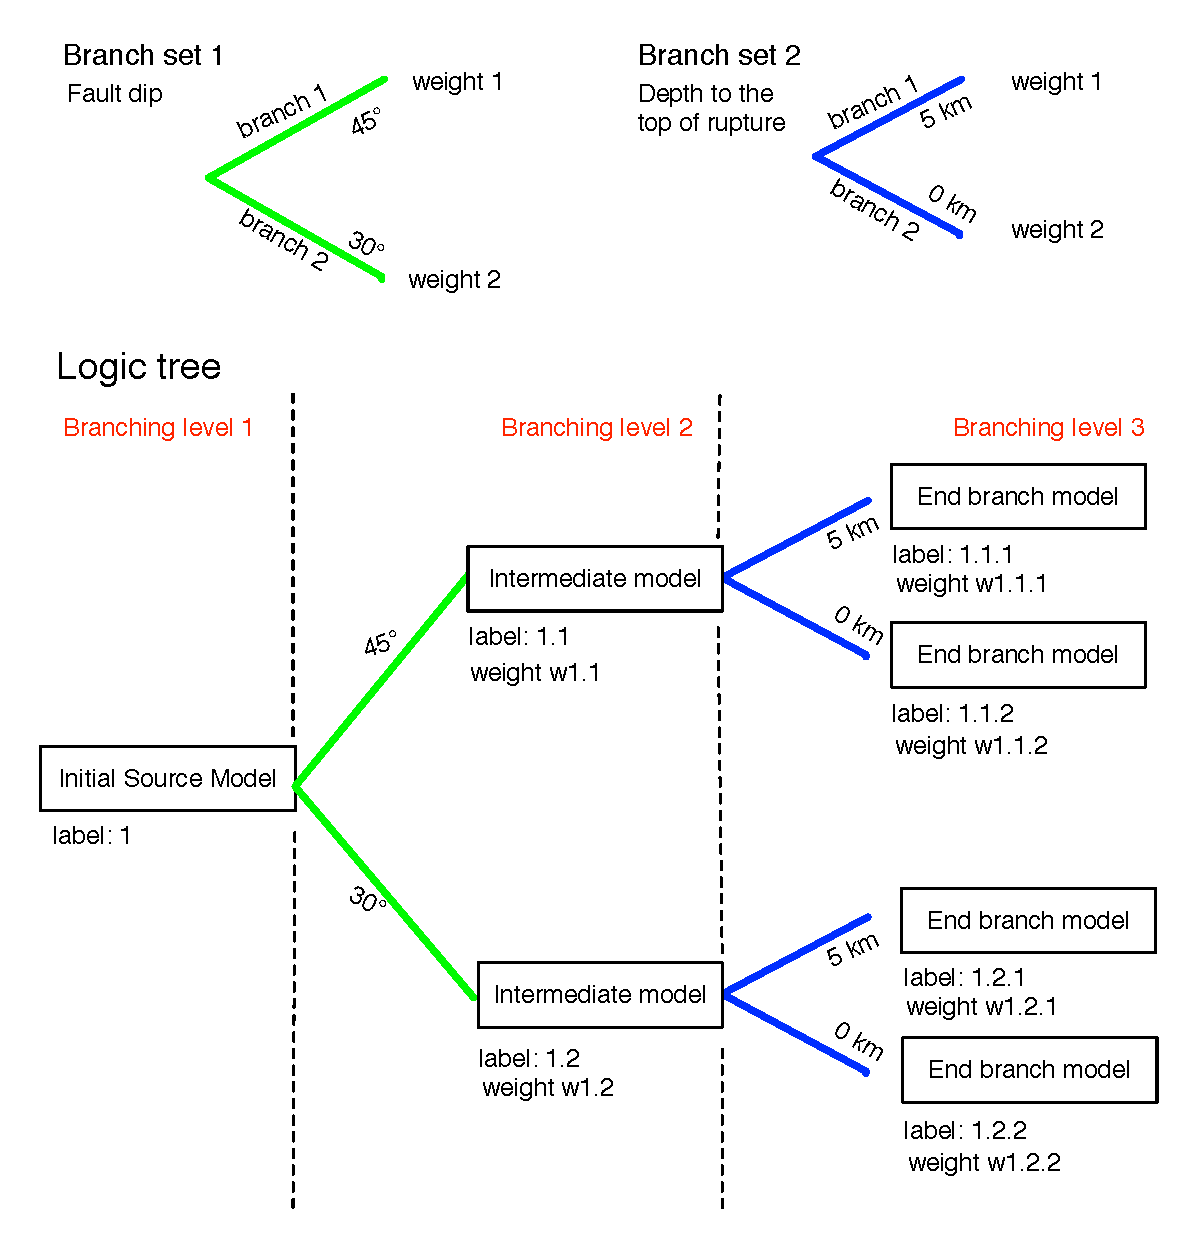
\includegraphics[width=15cm]{./Figures/Part_Hazard/logic_tree_schema.eps}
\caption{Example of a logic tree structure as defined in OpenQuake. The upper
part of the Figure depicts two branching levels.}
\label{fig:logic_tree_schema}
\end{figure}
% . . . . . . . . . . . . . . . . . . . . . . . . . . . . . . . . . . . < Figure
%

Figure \ref{fig:nrMl_logic_tree_example} shows an example of a nrML file 
describing the logic tree structure.
%
% . . . . . . . . . . . . . . . . . . . . . . . . . . . . . . . . . . . > Figure
\begin{figure}[!ht]
\small
\begin{Verbatim}[numbers=left,frame=single,fontsize=\small]
<?xml version="1.0" encoding="UTF-8"?>
</ns2:logicTreeSet>
\end{Verbatim}
\normalsize
\caption{nrML example}
\label{fig:nrMl_logic_tree_example}
\vspace*{1em}
\end{figure}
% . . . . . . . . . . . . . . . . . . . . . . . . . . . . . . . . . . . < Figure
%
% ------------------------------------------------------------------------------
\section[The OpenQuake source model]{The OpenQuake source model - Description 
of input data pertinent to the creation of the ERF}
%
The creation of the Earthquake Rupture Forecast (or seismicity probabilistic 
occurrence model) is the first step in the calculation of hazard following a 
probabilistic procedure. 

As mentioned in the introductory part of this Chapter, information describing 
the input data for the creating the ERF in OpenQuake is always organized into 
a logic tree structure.
%
%  - - - - - - - - - - - - - - - - - - - - - - - - - - - - - - - - - - - - - - -
\subsection{Seismic source typologies description}
\label{hazard:seismic_source_types}
%
OpenQuake, at present time, provides four seismic source typologies, for the 
most part defined in the course of the GEM1 project \citep{pagani2010}:
\begin{itemize}
\item Area source - This source type is the one that - at least for the time 
being - is most frequently adopted in national and regional PSHA models.
\item Grid source - Grid sources can be considered a replacement for area 
sources since they both model distributed seismicity;
\item Simple fault sources - Simple faults are the easiest modality available
to specify the parameters need to characterize a fault source. This typology
is usually adopted to describe shallow seismogenic fault sources.
\item Complex fault sources - Complex faults is usually adopted to model
subduction interface sources with a complex geometry. 
\end{itemize}

The basic assumptions adopted in the definition of these source typologies 
are the following:
\begin{itemize}
\item In the case of area and fault sources, the seismicity is homogeneously 
distributed over the source; 
\item Seismicity temporal occurrence follows a Poissonian model; 
\item The frequency-magnitude distribution can be approximated to a evenly 
discretized distribution. 
\end{itemize}
%
%  . . . . . . . . . . . . . . . . . . . . . . . . . . . . . . . . . . . . . . . 
\subsubsection{Area sources}
\label{hazard:seismic_source_types:areaSources}
\index{Source type!area} 
\index{Area source|see{Source type}}
Area sources usually model the seismicity occurring over wide areas where fault 
sources identification or characterization - i.e. the unambiguous definition 
of seismicity occurrence parameters - is difficult. 

The \citet{sshac1997} defined three main types of area seismic sources using as 
a discriminant their extension:
\begin{enumerate}
\item Area sources enclosing concentrated zones of seismicity;
\item Regional area sources;
\item Background area sources.
\end{enumerate}
As a general rule, the criteria - and the related uncertainties - adopted for 
their definition varies according to each area source type. From a hazard 
computation standpoint we do not introduce any difference between these three 
area types.
	\marginpar{marco: In the future we may support a specialized background 
	area source type}
%
%  . . . . . . . . . . . . . . . . . . . . . . . . . . . . . . . . . . . . . . . 
\paragraph{Parameters}
\begin{itemize}
\item A polygon that identifies the external border of the area. Eventually, 
internal borders can be specified so as to create holes inside an area.
	\marginpar{marco: I don't think nrML supports area sources with holes.}
\item One (or many) couples of the following objects:
\begin{itemize}
	\item A discrete Frequency-Magnitude Distribution (FMD)
	\item Strike, dip, and rake angles characterizing the seismicity specified 
	in the associated FMD and occurring in the area source under consideration. 
	For example, \cite{coppersmith2009} defines a discrete 
	distribution of strike values (dip is not considered because the source-site 
	metrics they use is the Joyner-Boore distance). 
\end{itemize}
This area source specification permits the accurate characterization of 
seismicity occurrence within an area by explicitly distributing the seismicity 
on the existing faulting trends. 
\item An array to specify the depth to the top of rupture dependency on magnitude. 
The array contains two columns and one or many $<$depth, magnitude$>$ tuples. 
Each tuple specifies the depth to the top of rupture for magnitudes equal or 
greater than the specific value. 
\item A value to indicate the hypocentral depth in case of punctual sources. 
By convention all the events with magnitude lower than the lowest value contained 
in the array used to specify the depth to the top of rupture are modelled 
considering a punctual source. On the opposite, ruptures with magnitude equal or 
greater than the lowest value of magnitude contained in the depth to the top of 
rupture array are modelled considering their finite dimensions. 
\end{itemize}
%
%  . . . . . . . . . . . . . . . . . . . . . . . . . . . . . . . . . . . . . . .
\subsubsection{Grid sources}
\index{Source type!grid}
\index{Grid source|see{Source type}}
A grid source  is a typology used to model distributed seismicity - usually of low and intermediate magnitude.

Grid sources can be considered as a PSHA source model alternative to area 
sources since they both try to represent distributed seismicity. Grid sources 
usually derive from the application of seismicity smoothing algorithms 
\citep{frankel1995,woo1996}. 

The use of these algorithms carries some advantages compared to area sources, 
indeed, (1) they remove most of the unavoidable degree of subjectivity due to 
the definition of the geometries and (2) they define a seismicity spatial 
pattern that is, usually, more similar to reality. Nevertheless, some smoothing 
algorithms require the a-priori definition of some setup parameters that expose 
the calculation to a certain partiality level.

Grid source models are modelled in OpenQuake simply as set of 
point sources. The next section describes the parameters required to 
characterize a point source.
%
%  . . . . . . . . . . . . . . . . . . . . . . . . . . . . . . . . . . . . . . . 
\paragraph{Parameters}
%
For each grid node:
\begin{itemize}
\item A location specified in terms of the $<$latitude,longitude$>$ tuple;
\item Similarly to area sources, one (or many) couples of the following objects:
	\begin{itemize}
	\item A discrete Frequency-Magnitude Distribution (FMD)
	\item Strike, dip, and rake angles characterizing the seismicity specified 
	in the associated FMD. 
	\end{itemize}
\item An array to specify the dependency on magnitude of the depth to the top of 
	rupture. This array contains two columns and one or many 
	$<$depth, magnitude$>$ tuples where each tuple specifies the depth to the 
	top of rupture for magnitudes equal or greater than a specific value. 
\item A value to indicate the hypocentral depth in case of punctual sources. The 
	same convention specified for area sources applies here. 
\end{itemize}
%
%  - - - - - - - - - - - - - - - - - - - - - - - - - - - - - - - - - - - - - - - 
\subsection{Accounting for rupture finiteness in case of areal and grid sources}
%
In the scientific literature is well known that for magnitudes approximately 
greater than six the finite dimension of the rupture cannot be neglected in 
the calculation of the source-site distance. 
	\marginpar{marco: we need at least one citation}
	\marginpar{marco: it's not clear if and how much ruptures can extend
	outside the area border}

To correctly calculate the source-site distance in case of area and grid sources 
two are the approaches available. The first is to multiply the epicentral or 
hypocentral distance by a correction factor (see for example \cite{harmsen2008})
the second requires to place on each node a number of ruptures with different 
orientation. 
%
%  . . . . . . . . . . . . . . . . . . . . . . . . . . . . . . . . . . . . . . .
\subsubsection{Simple faults}
\index{Source type!fault!simple geometry} 
\index{Simple fault|see{Source type}}
%
Simple Faults are the most common source type used to model faults; the 
``simple'' adjective here refers to the geometry description of the source 
which is basically obtained by projecting a trace along a representative dip 
direction. 
%
%  .   .   .   .   .   .   .   .   .   .   .   .   .   .   .   .   .   .   .   . 
\paragraph{Parameters}
%
\begin{itemize}
\item A fault trace (usually a multi-segment line) 
\item A FMD 
\item A representative value of the dip angle (Aki-Richards convention; see 
	\citet{aki2002}),
\item Rake angle (Aki-Richards convention; see \citet{aki2002}) 
\item Upper and lower values of depth limiting the seismogenic interval 
\item A boolean flag that specifies if ruptures should follow a magnitude scaling 
relationship and thus be distributed homogeneously over the fault surface or it is 
accepted that ruptures of whatever magnitude (of course of the ones admitted by 
the FMD) will rupture the whole fault surface.
\end{itemize}
%
%  . . . . . . . . . . . . . . . . . . . . . . . . . . . . . . . . . . . . . . .
\subsubsection{Complex faults}
\index{Source type!fault!complex geometry}
\index{Complex fault|see{Source type}}
%
Complex faults  differ from simple fault just by the way geometry is described and, consequently in the way the fault surface is created. The input parameters used to describe complex faults are, for the most part, the same used to describe the simple fault typology. In particular, in the case of complex faults the dip angle is not requested while the fault trace is substituted by two fault traces used to limit at top and bottom the fault surface. 
%
%  .   .   .   .   .   .   .   .   .   .   .   .   .   .   .   .   .   .   .   . 
\paragraph{Representation of complex faults}
%
Usually, we use complex faults to model intraplate megathrust faults such as the 
big subduction structures active in the Pacific (Sumatra, South America, Japan).

%
% ------------------------------------------------------------------------------
\section{GMPEs description}
\label{hazard:gmpe_selection}
%

%
% ------------------------------------------------------------------------------
\section{Calculation settings description}
\label{hazard:calculation_settings}
%



